\chapter{Semantic Graph Matching for Multimodal Reasoning with MGRAG}
\label{ch:mgrag}

This chapter is based on \emph{MGRAG: Semantic Subgraph Matching and Graph-Aware Caching for Multimodal Retrieval-Augmented Generation}, published in the \emph{Proceedings of the VLDB Endowment}, volume 19, number 9, pages 2480--2493, 2026~\cite{mgrag-paper}. It studies how a query can determine the evidence graph to construct, how paths can express semantic correspondences across different graph topologies, and how the resulting structure can guide context computation.

\section{Multimodal Evidence and Query Requirements}
\label{sec:mgrag:problem}

An answer to a multimodal query may depend on a relation that is distributed across text and images. A document can name a person, an image can show an action, and another passage can connect that person to an event. Retrieving each item by its similarity to the query supplies candidate evidence, but the relation needed for the answer can remain implicit. A graph makes the entities and their connections available as a retrieval object. Its usefulness depends on which facts are extracted and on whether its representation can express the relation requested by the query.

This chapter considers a corpus $\mathcal D=\mathcal D_{\mathrm{txt}}\cup\mathcal D_{\mathrm{img}}$ and a query $q$ that can contain text, an image, or both. A retrieval module selects evidence from the corpus, and a multimodal language model generates an answer using that evidence. The research question is how to construct and retrieve a query-relevant relational representation while controlling the cost of preparing and processing the context. The answer-generation task remains grounded in the original documents and images. The graph supplies an additional representation of their query-related content.

Three decisions govern this process. The first concerns when to construct a graph. A corpus-wide graph requires extraction before the query is known. Its entities and relations consequently reflect the extraction prompt's general description of the corpus. When an image contains several people, objects, and actions, the details relevant to one query can differ from those relevant to another. MGRAG places the query inside the extraction process and constructs the graph incrementally from ranked evidence. The graph is specific to the current query.

The second decision concerns what constitutes a match. A query and its supporting documents need not use the same decomposition of a fact. The published motivating example describes a data graph containing two \texttt{father\_of} edges and a query containing one \texttt{grandfather\_of} edge. The requested relation is represented by a two-hop path in the data. Requiring the same edge topology would exclude this correspondence. Figure~\ref{fig:mgrag:motivation} reproduces the example. MGRAG evaluates semantic representations of paths so that a query relation can be supported by a sequence of evidence relations.

\begin{figure}[tbp]
\centering
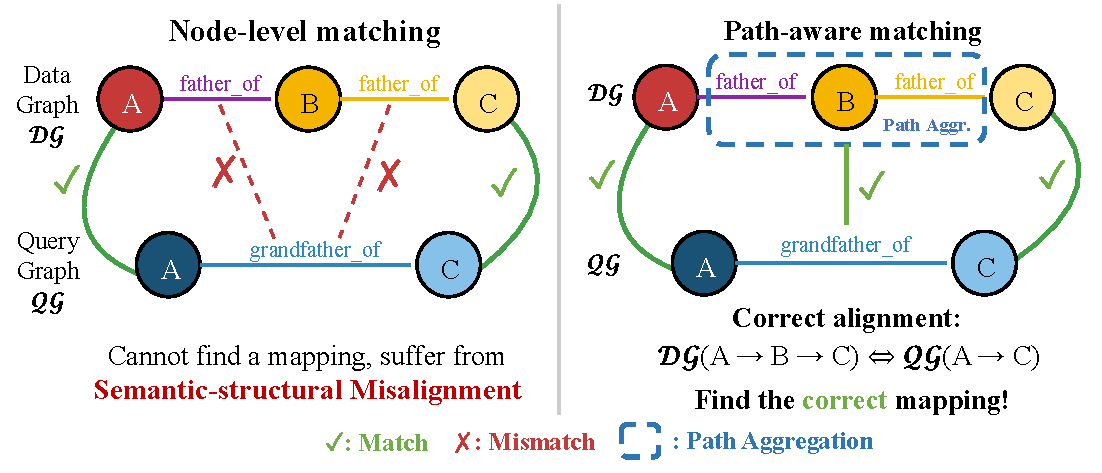
\includegraphics[width=0.85\textwidth]{figures/mgrag/motivation.pdf}
\caption{Path-level correspondence in the MGRAG motivating example. A \texttt{grandfather\_of} relation corresponds to two \texttt{father\_of} edges. Original Figure 1, p.~2481~\cite{mgrag-paper}.}
\label{fig:mgrag:motivation}
\end{figure}

The third decision concerns the cost of processing retrieved evidence. Graph construction already sends evidence to a language model to extract entities and relations. Some of that content appears again when the matched graph and its source chunks are used for answering. Reusing the earlier key-value (KV) states can reduce repeated computation. Their suitability depends on the new query and context, so MGRAG selectively recomputes token states. It combines attention scores with topological features of the facts associated with those tokens. Structure thus enters both evidence selection and the subsequent use of the selected context.

These decisions extend the thesis from connected textual evidence to multimodal evidence whose semantic decomposition is query-dependent. MGRAG develops its own graph construction, path-matching procedure, and cache score. The connection to the preceding studies lies in the role of explicit structure in organizing evidence. The evaluation in this chapter measures multimodal answer quality and context-serving costs under the published MGRAG protocol.

\section{Framework and Evidence Representations}
\label{sec:mgrag:overview}

Figure~\ref{fig:mgrag:pipeline} shows three stages. Coarse-grained ranking orders text chunks and images according to their relevance to the query. Fine-grained retrieval consumes this ranked list, extracts query-related facts, and searches the growing graph for a semantic match. Graph-aware KV recomputation then determines which cached token states to update for answer generation. The stopping decision in the middle stage connects ranking, graph construction, and matching. Each additional chunk can change whether the graph contains a suitable correspondence.

\begin{figure}[tbp]
\centering
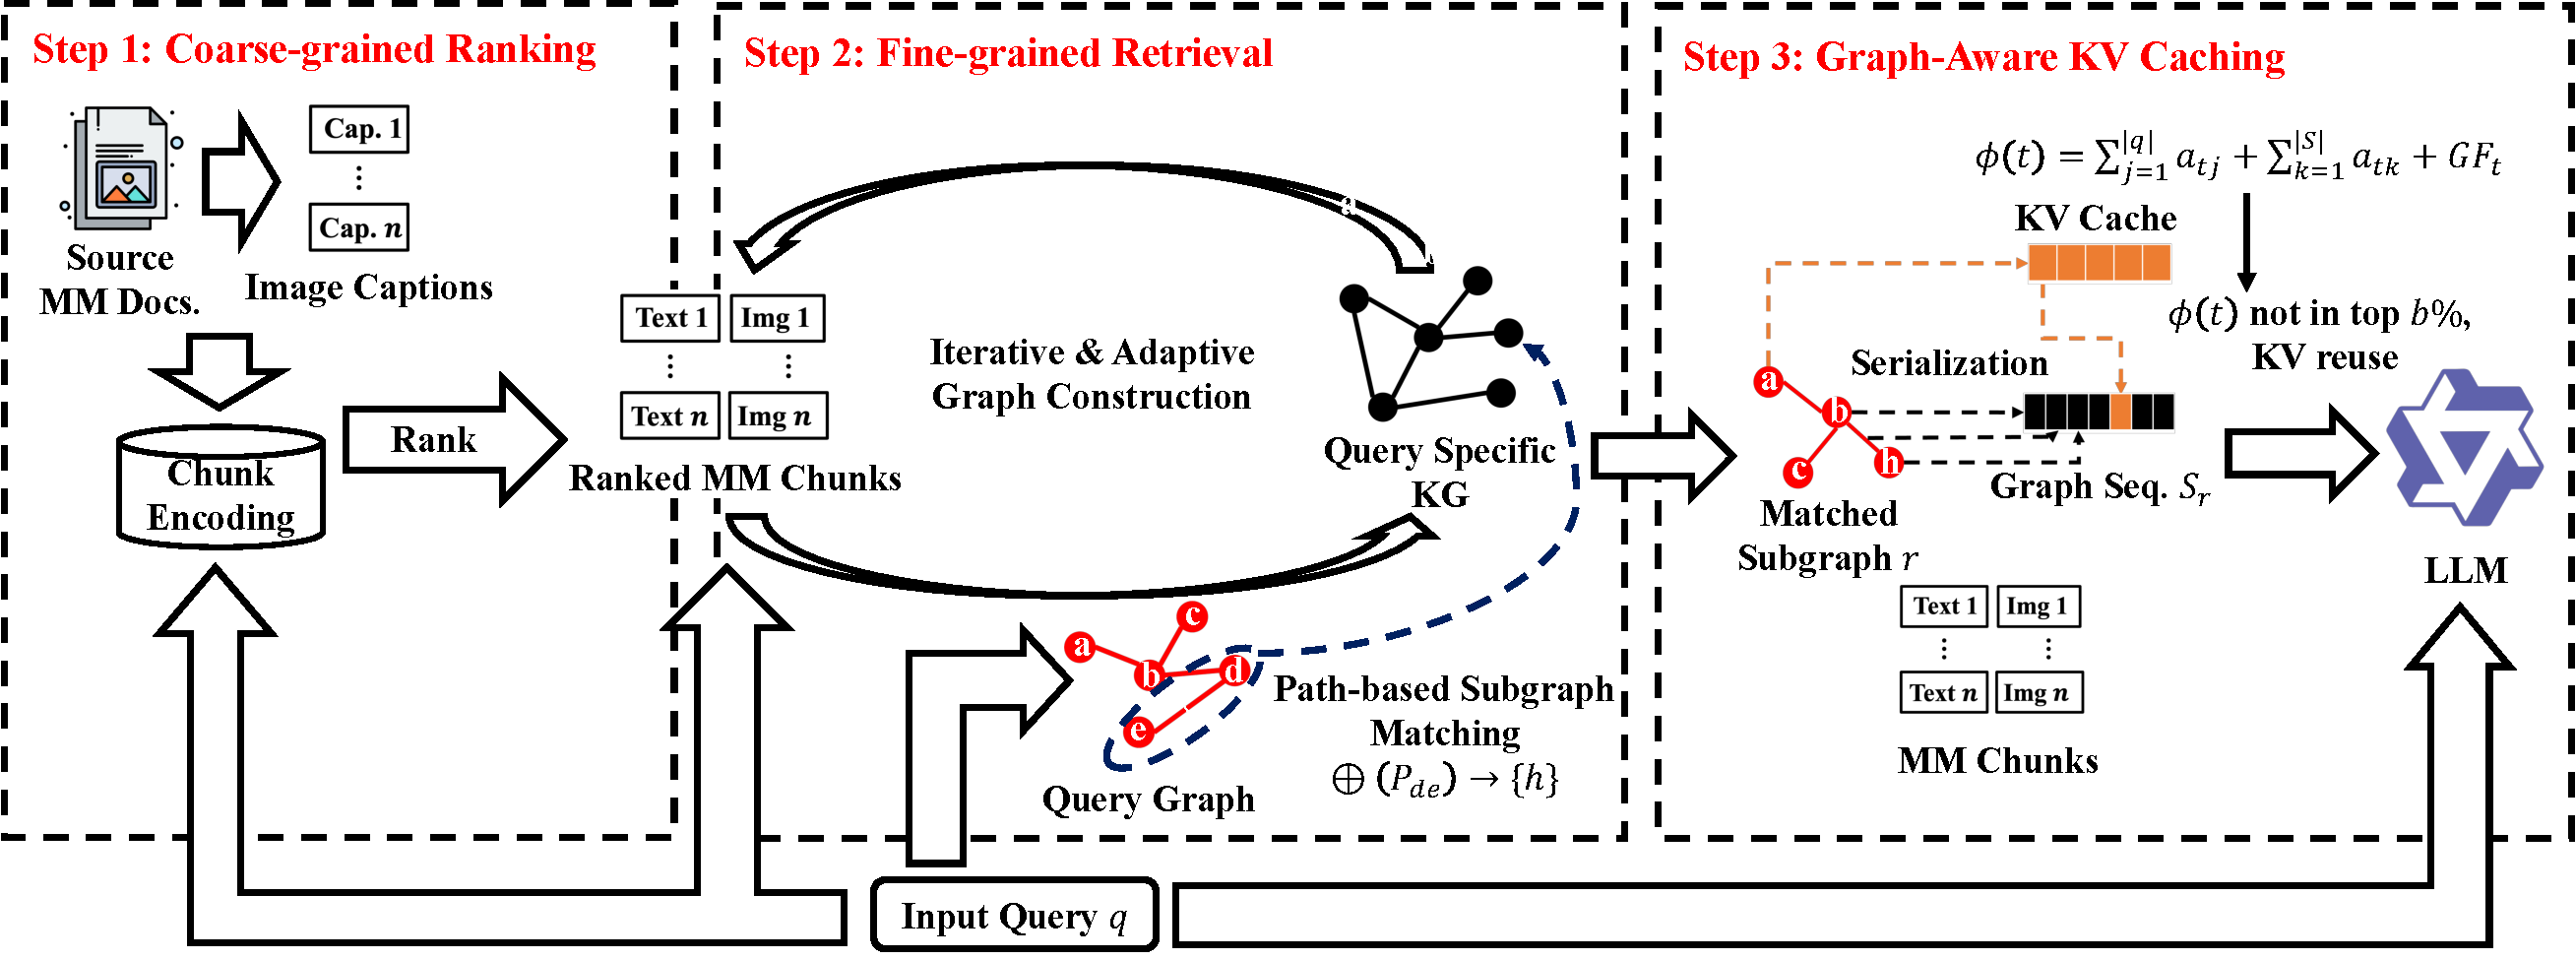
\includegraphics[width=\textwidth]{figures/mgrag/pipeline_new.pdf}
\caption{The MGRAG pipeline. Ranked chunks support incremental query-aware graph construction and path-based matching. The matched graph also supplies features for selective KV recomputation. Original Figure 2, p.~2484~\cite{mgrag-paper}.}
\label{fig:mgrag:pipeline}
\end{figure}

Two graphs serve different purposes. The query graph $\mathcal{QG}_q=(\widehat{\mathcal V}_q,\widehat{\mathcal E}_q)$ describes the entities and relations requested by $q$, including placeholders for unknown information. The evidence graph $\mathcal{KG}_q=(\mathcal V_q,\mathcal E_q)$ contains facts extracted from the chunks considered for that query. A mapping connects query entities to evidence entities. Paths between the mapped endpoints supply candidate evidence for the query relations.

For generation, MGRAG uses the graph sequence $S_r$, the original chunks $\mathcal C_q$ consumed during construction, and the query $q$. Keeping the chunks preserves access to text and visual evidence beyond the extracted triples. Their identity also links the selected graph to the material originally ranked and processed during construction. The graph gives the generator an explicit selection of relational content, while the source chunks provide the material from which the selection was made. The final multimodal context retains the original images alongside their extracted relational representation.

\section{Coarse-grained Ranking}
\label{sec:mgrag:ranking}

MGRAG first divides textual documents into overlapping chunks. The published setting uses a chunk length $l_c=256$ tokens and overlap $l_o=32$ tokens. Images form the other members of the chunk collection, giving $\mathcal C=\mathcal T\cup\mathcal D_{\mathrm{img}}$, where $\mathcal T$ denotes the text chunks. This collection is the input to the coarse retrieval stage. Ranking identifies the order in which content will be examined, rather than directly defining the final graph context.

The implementation uses the text encoder bge-base-en-v1.5~\cite{mgrag-bge_embedding}. Text chunks are encoded directly. An image is represented for ranking by its caption, which can be supplied by the dataset or generated by a language model. Both types of evidence can therefore be compared in the text embedding space. Let $\mathcal M$ denote that encoder and $\mathbf h_c$ the representation of a candidate chunk. For an image chunk, the input to $\mathcal M$ is its caption. This detail matters because the ranking representation expresses the image through language, whereas the later extraction and answering stages can use its visual content.

For a query containing text $q_{\mathrm{txt}}$ and an image caption $q_{\mathrm{cap}}$, MGRAG averages the two representations,
\begin{equation}
\mathbf h_q=\frac{\mathcal M(q_{\mathrm{txt}})+\mathcal M(q_{\mathrm{cap}})}{2}.
\label{eq:mgrag:query-embedding}
\end{equation}
A query with one modality uses its corresponding textual representation. The distance to a candidate is
\begin{equation}
 d(q,c)=\lVert\mathbf h_q-\mathbf h_c\rVert_2,
\label{eq:mgrag:distance}
\end{equation}
and the chunks are ordered by increasing distance. Equations~\ref{eq:mgrag:query-embedding} and~\ref{eq:mgrag:distance} retain the averaging and Euclidean-ranking operations of the published method.

This stage gives a query-dependent priority to relatively inexpensive chunk representations. Fine-grained processing begins with the nearest chunk and can move down the list when its current graph is insufficient. A high-ranked chunk becomes a candidate for relational extraction and subsequent matching. Conversely, graph matching can stop construction before every candidate has been processed. The coarse-to-fine design separates the cost of ordering the corpus from the cost of extracting its query-related facts.

Caption quality affects which images receive an early position. A caption can omit a visual detail that becomes relevant during graph construction, or foreground content unrelated to the query. The published CLIP substitution experiment tests an alternative coarse representation within this pipeline. Its results are discussed alongside the component ablations in Section~\ref{sec:mgrag:ablations}, where the encoder choice can be assessed under the same answering task.

\section{Query-aware Graph Construction}
\label{sec:mgrag:construction}

\subsection{Representing the query}

MGRAG asks the language model to extract entities and relations from the query. Some query entities are known, such as the name of a person or an object appearing in the question. Others are requested by the question. The extraction prompt represents those unknown components using semantically meaningful placeholders, including types such as \emph{Person} or \emph{Year}. A placeholder provides a textual representation that can be compared with evidence entities even though its value has not yet been supplied.

Figure~\ref{fig:mgrag:query-graph} shows the query and evidence graph representations. The placeholder boxes describe missing knowledge in the query. Passage nodes connect extracted entities back to their chunks. These connections let the graph carry both relational content and its association with the original multimodal evidence. In a multimodal corpus, a passage node can represent an image as well as a text chunk.

\begin{figure}[tbp]
\centering
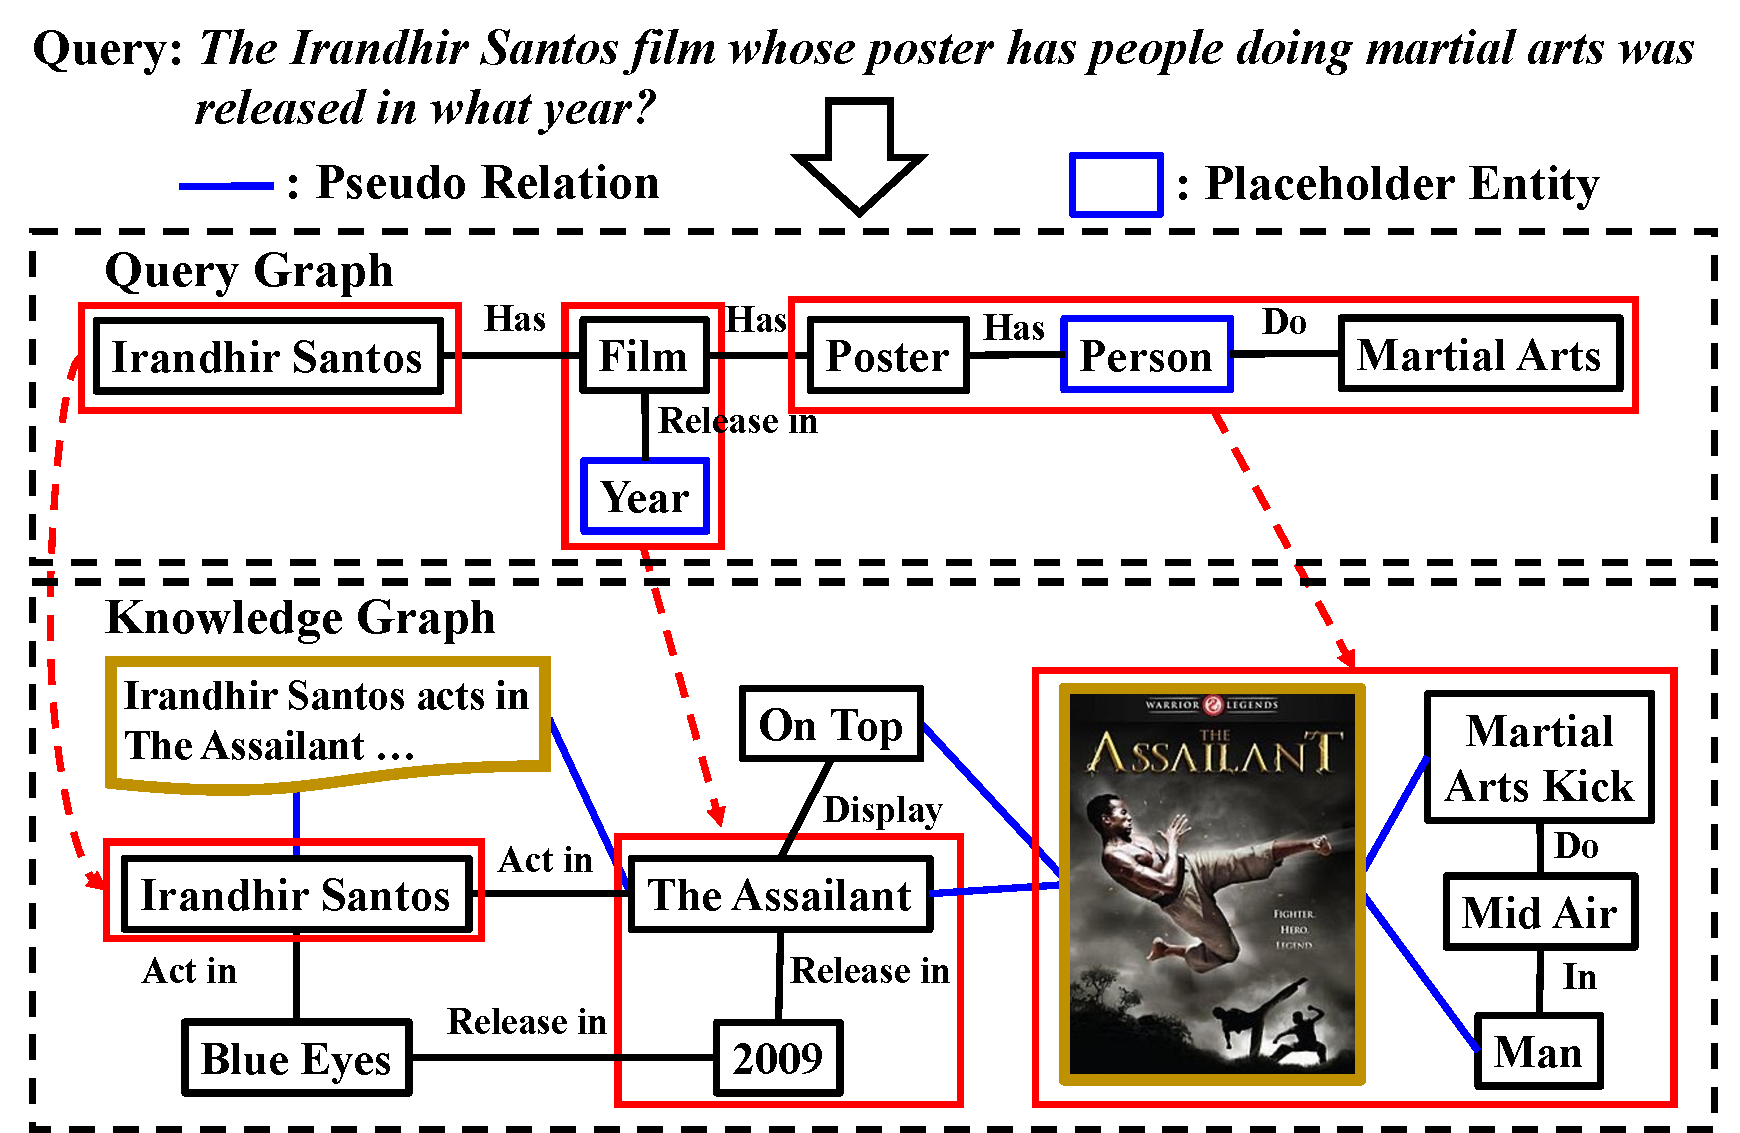
\includegraphics[width=0.95\textwidth]{figures/mgrag/query_graph.pdf}
\caption{Query and evidence graphs in path-based semantic matching. Placeholder entities express unknown query information; pseudo-relations connect passage nodes to extracted entities. Original Figure 3, p.~2485~\cite{mgrag-paper}.}
\label{fig:mgrag:query-graph}
\end{figure}

The original example asks which year an Irandhir Santos film was released when its poster shows people doing martial arts. The query graph connects the actor to an unknown film, the film to a poster, and a person on the poster to an action. It also includes a release-year requirement. The evidence graph contains named film candidates and a visual description of a man performing a martial-arts kick in midair. The depicted film, \emph{The Assailant}, is connected to the year 2009.

The example separates identifying the film from reading its release year. The actor's name alone can lead to several film candidates, including the other film shown in the graph. The visual relation supplies the condition that distinguishes the requested candidate. Once the candidate is connected to the poster evidence, the release relation provides the requested value. The query therefore needs a connected account of the actor, film, depicted action, and year. A list containing a similar actor passage and an unrelated year passage would leave that correspondence unresolved.

The placeholders give the matcher explicit locations for these missing values. The film placeholder can be compared with named film entities, while the year placeholder marks the relation whose endpoint supplies the requested answer. Representing unknown values by their semantic roles lets matching operate before those values are known. The path procedure then tests whether the selected evidence entities are connected through semantically suitable relations. This is the point at which the query's information requirement becomes a constraint on the retrieved graph.

The query graph expresses a retrieval requirement at entity and relation granularity. Its construction is a model-mediated interpretation of the question. The downstream matcher operates on this interpretation, including the wording chosen for placeholders and relations. A semantic match therefore indicates agreement between the represented query and represented evidence. Answer quality is evaluated separately using the original question and reference answer.

\subsection{Extracting facts from ranked chunks}

For a chunk $c$, the extraction model receives the chunk, query, and extraction prompt $p_{\mathrm{ext}}$. Its output contains query-related entities and relations,
\begin{equation}
 (\mathcal V_q^c,\mathcal E_q^c)
 =\operatorname{LLM}(c,q,p_{\mathrm{ext}}).
\label{eq:mgrag:extraction}
\end{equation}
Including $q$ makes the extraction selective. The model is asked to identify events and relations relevant to the current question, rather than to enumerate every describable fact in the chunk. For an image, this permits attention to query-related visual events; for text, it permits selection of the entities and relationships needed to describe the requested evidence.

The chunk is also added as a passage node. MGRAG connects this node to the entities extracted from it using the pseudo-relation \texttt{consists\_in}, retaining the published relation name and orientation from chunk to entity. If $\mathcal C_q^{(i)}$ is the prefix of ranked chunks consumed after iteration $i$, the cumulative graph contains
\begin{align}
 \mathcal V_q^{(i)}
 &=\bigcup_{c\in\mathcal C_q^{(i)}}(\mathcal V_q^c\cup\{c\}),\\
 \mathcal E_q^{(i)}
 &=\bigcup_{c\in\mathcal C_q^{(i)}}\left(\mathcal E_q^c\cup
 \{(c,\texttt{consists\_in},v):v\in\mathcal V_q^c\}\right).
\label{eq:mgrag:graph-union}
\end{align}
The iteration-indexed notation makes explicit that the unions range over the chunks already processed. 

Passage nodes give the matcher a route between a fact and its context. They can also connect facts associated with the same source item. The resulting graph combines extracted semantic relations with document-membership relations. These two edge types have different interpretations, even though both participate in the evidence representation. The distinction is visible in the original example's use of separate edge colors.

\subsection{Matching as a stopping decision}

After each graph update, MGRAG attempts path-based semantic subgraph matching against the query graph. A valid match ends the construction loop. If the matcher returns an empty result, the next ranked chunk is used to enrich the graph. The loop is bounded by the maximum number of construction iterations $\mu$. Thus, the amount of graph construction depends on both the ranking order and the matching outcome.

This design uses semantic coverage as an operational stopping test. Coverage is evaluated through the query graph's entities and relations, so a match requires more than one highly similar isolated entity. The procedure seeks a correspondence for the query's relational requirements. When the current graph lacks such a correspondence, additional evidence can introduce a missing endpoint, a relation, or a path between existing endpoints. The graph can therefore become matchable through information accumulated across chunks.

The iteration cap controls the amount of evidence examined. It also bounds the opportunity to recover a fact that occurs late in the ranking. Reaching the cap and finding a valid match are distinct termination events. The matcher returns an empty result when its search finds no valid correspondence in the current graph. The cap, graph extraction, and matching threshold jointly determine which context reaches the answer generator.

\section{Path-based Semantic Subgraph Matching}
\label{sec:mgrag:matching}

\subsection{From edges to paths}

A relation in the query graph can be expressed by several relations in the evidence graph. MGRAG assigns text embeddings to entity and relation descriptions. For a path $P(u,v)$ containing relations $r_1,\ldots,r_k$, it defines a semantic representation by aggregating the relation embeddings,
\begin{equation}
 \mathbf h_{P(u,v)}=\bigoplus_{j=1}^{k}\mathbf h_{r_j}.
\label{eq:mgrag:path-embedding}
\end{equation}
The aggregation operator can use mean pooling. This operation provides a representation of the composed evidence relation that can be compared with a query relation. The published greedy expansion further evaluates a joint representation containing the current path, candidate edge, and candidate endpoint. These are the path representation and extension test used at different steps of the procedure.

Let $I:\widehat{\mathcal V}_q\rightarrow\mathcal V_q$ be a candidate entity mapping. For a query edge $(u,\widehat r,v)$, the candidate evidence paths run from $I(u)$ to $I(v)$. Denote this collection by $\mathcal P(I(u),I(v))$. The matching objective is
\begin{equation}
\max_I\ \sum_{(u,\widehat r,v)\in\widehat{\mathcal E}_q}
 \max_{P\in\mathcal P(I(u),I(v))}
 \cos(\mathbf h_{\widehat r},\mathbf h_P).
\label{eq:mgrag:matching-objective}
\end{equation}
Candidate mappings must satisfy the semantic threshold $\theta$ for the mapped entities and for every query relation's supporting path,
\begin{align}
 \cos(\mathbf h_u,\mathbf h_{I(u)})&>\theta
 &&\text{for all }u\in\widehat{\mathcal V}_q,\\
 \max_{P\in\mathcal P(I(u),I(v))}\cos(\mathbf h_{\widehat r},\mathbf h_P)&>\theta
 &&\text{for all }(u,\widehat r,v)\in\widehat{\mathcal E}_q.
\label{eq:mgrag:matching-constraints}
\end{align}
The constraints validate each query edge against an associated evidence path. The selected evidence is the subgraph formed from the mapped entities and accepted paths, which can include intermediate entities absent from the query graph.

For a fixed candidate mapping, the inner maximization in Equation~\ref{eq:mgrag:matching-objective} selects a supporting path for each query relation. The outer search compares entity mappings after those relation scores have been obtained. These levels distinguish the problem of locating the query's entities from the problem of explaining their relationships. Two mappings can have similar endpoint embeddings yet differ in whether their connecting paths satisfy the requested relation. Conversely, several paths between the same mapped endpoints can express different relations and receive different semantic scores.

The returned subgraph is assembled from the paths needed by the accepted query edges. Paths can share intermediate entities and edges. Their union exposes those shared facts in the evidence graph, while the query graph continues to specify which relational requirements were validated. A graph assembled in this way need not have the same number of entities as the query graph. Intermediate evidence nodes are precisely what permits a relation expressed compactly in the question to be supported by a more detailed description in the corpus.

This representation relaxes the requirement that the two graphs express a fact with the same number of edges. In the family-relation example, the evidence path has two steps and the query relation has one. Their correspondence is judged through semantic similarity. The procedure retains endpoint requirements, so the selected relation must connect entities that themselves correspond to the query. It combines entity-level alignment with path-level evidence instead of treating either component as sufficient on its own.

\subsection{Anchor selection and candidate mappings}

MGRAG first computes pairwise cosine similarities between query entities and evidence entities. The highest-similarity pair supplies an anchor entity in the query graph and its candidate counterpart in the evidence graph. If no valid match is obtained from that anchor, the method tries other anchors. For the selected query anchor, Algorithm~\ref{alg:mgrag:matching} considers each evidence counterpart exceeding the threshold and enumerates mappings consistent with that correspondence.

Candidate mappings are enumerated using a similarity-based modification of VF2~\cite{mgrag-cordella2004sub}. VF2 supplies a graph-matching search procedure; the MGRAG adaptation uses the threshold $\theta$ in semantic feasibility checks. Each candidate is then validated relation by relation through greedy path search. A candidate entity correspondence can consequently be rejected because one of its required relations lacks an acceptable evidence path.

For each accepted mapping, the algorithm takes the union of the paths that support its query edges. It averages the edge-wise semantic similarities to obtain a score $s$. The highest-scoring accepted subgraph is returned. Dividing by the number of query edges does not change the ranking of candidate mappings for the same query. It provides an average semantic score with a common range across queries whose graph sizes differ.

\begin{algorithm}[tbp]
\caption{Path-based semantic matching in MGRAG}
\label{alg:mgrag:matching}
\begin{algorithmic}[1]
\REQUIRE Query graph $\mathcal{QG}_q$, query anchor $\gamma$, evidence graph $\mathcal{KG}_q$, threshold $\theta$
\STATE Initialize valid results $\mathcal R\gets\varnothing$
\FOR{each $v_a\in\mathcal V_q$ with $\cos(\mathbf h_{v_a},\mathbf h_\gamma)>\theta$}
\STATE Enumerate candidate mappings consistent with $I(\gamma)=v_a$
\FOR{each candidate mapping $I$}
\STATE Initialize the subgraph with mapped query entities; set $s\gets0$
\FOR{each query edge $(u,\widehat r,v)$}
\STATE Search greedily for a semantically valid path from $I(u)$ to $I(v)$
\IF{the path search fails}
\STATE Reject $I$ and stop validating this mapping
\ELSE
\STATE Add the path's nodes and edges to the candidate subgraph
\STATE Add its cosine similarity to $s$
\ENDIF
\ENDFOR
\IF{every query edge has a valid path}
\STATE Add the subgraph and score $s/|\widehat{\mathcal E}_q|$ to $\mathcal R$
\ENDIF
\ENDFOR
\ENDFOR
\STATE Return the highest-scoring result, or $\varnothing$ if $\mathcal R$ is empty
\end{algorithmic}
\end{algorithm}

\subsection{Greedy semantic path growth}

The path search begins at the mapped source entity and maintains its current endpoint $x$. For each neighboring entity $y$ and connecting edge $(x,r,y)$, MGRAG evaluates the candidate extension using
\begin{equation}
 \cos\!\left(\mathbf h_P\oplus\mathbf h_{e(x,r,y)}\oplus\mathbf h_y,
 \mathbf h_{\widehat e(u,\widehat r,v)}\right).
\label{eq:mgrag:greedy-score}
\end{equation}
Among extensions exceeding $\theta$, it selects the highest-scoring one, appends that edge to the path, and updates the endpoint to $y$. This repeats until the path reaches the mapped target. The search fails when no qualifying extension is available. The experiments also impose a maximum path length $l_p$ to bound expansion.

The endpoint and threshold checks serve different roles. Reaching the target gives the evidence path the required relational endpoints. Passing the semantic checks gives it a representation consistent with the requested relation. An attractive local extension can still prevent the greedy search from reaching the target, so a failed search does not establish that all possible paths fail. The algorithm returns the best result among the valid candidates it finds.

All query edges must pass path validation before a mapping is accepted. This condition prevents a single high-scoring relation from compensating for an unsupported required relation. The selected subgraph may contain paths of different lengths, because the evidence required by different query edges can have different decompositions. Construction then stops on that accepted match; otherwise, a further ranked chunk is incorporated and matching is attempted again.

\subsection{Published algorithmic properties}

The publication states that path-based semantic subgraph matching is NP-hard. Its proof sketch reduces subgraph isomorphism to a restricted instance with uniform embeddings and unit path lengths. The result motivates the use of semantic path growth and constrained mapping enumeration. The complexity of enumerating mappings remains relevant even when each individual extension is selected greedily.

The published Theorem 2 gives a threshold-based quality condition for a valid returned match. Every matched query relation has a supporting path with cosine similarity at least $\theta$. Under the strict acceptance test in Equation~\ref{eq:mgrag:matching-constraints}, the average score of an accepted mapping exceeds $\theta$ as well. This condition describes the semantic validation of returned evidence. It is conditional on finding a valid match and does not require the algorithm to recover one whenever such a subgraph exists.

The technical report discusses the threshold in terms of a bottleneck transport cost~\cite{mgrag-tech-report}. With a per-edge cost of one minus cosine similarity, the threshold limits the largest accepted local cost. The explicit theorem statement in the publisher PDF is used here to specify the result. The method's empirical quality is assessed by the graph-matching substitutions and answer-quality measurements in Section~\ref{sec:mgrag:results}.

\subsection{Serializing selected evidence}

After matching, MGRAG serializes the selected triples into $S_r$, separating facts with \texttt{[SEP]}. This sequence is combined with $q$ and the original chunks consumed during construction. The serialization supplies an explicit list of entities and relationships to the answering model. Original chunks remain available because extraction is a selective description of the evidence, and some linguistic or visual details may lie outside the triples.

The same entities and relations were involved in the earlier graph-construction calls. Their tokens can therefore overlap with tokens in the answering context. MGRAG uses this relationship to reuse cached computation from construction while updating states important to the new answering context. The graph produced during retrieval thus becomes an input to the context-computation policy as well as to the language model's prompt.

\section{Graph-aware KV Recomputation}
\label{sec:mgrag:cache}

\subsection{Reuse and selective updates}

A transformer caches key and value projections so that earlier token states can be reused. In MGRAG, content processed during graph construction appears again in the query-answering context. Recomputing every state repeats part of this work. Reusing every state can retain representations calculated under a different surrounding sequence. The cache policy chooses a subset for recomputation and reuses the others.

Let $\phi(t)$ be the recomputation score of token $t$. At each transformer layer, MGRAG recomputes the tokens in the highest $b\%$ of scores and reuses the cached states for the remaining tokens. The published description uses a fixed-size cache with least-recently-used eviction. Its proposed policy concerns the ranking of token states for selective recomputation. The budget is represented by $b$; the numerical experiment tables do not specify a fixed value for that budget.

Figure~\ref{fig:mgrag:cache} shows how the graph contributes. Query-related events are represented by entities and relations. The score combines attention to the query, attention to the graph sequence, and a feature derived from the topology of the associated fact. The goal of the added term is to give tokens access to an event-level structural signal alongside token-level attention.

\begin{figure}[tbp]
\centering
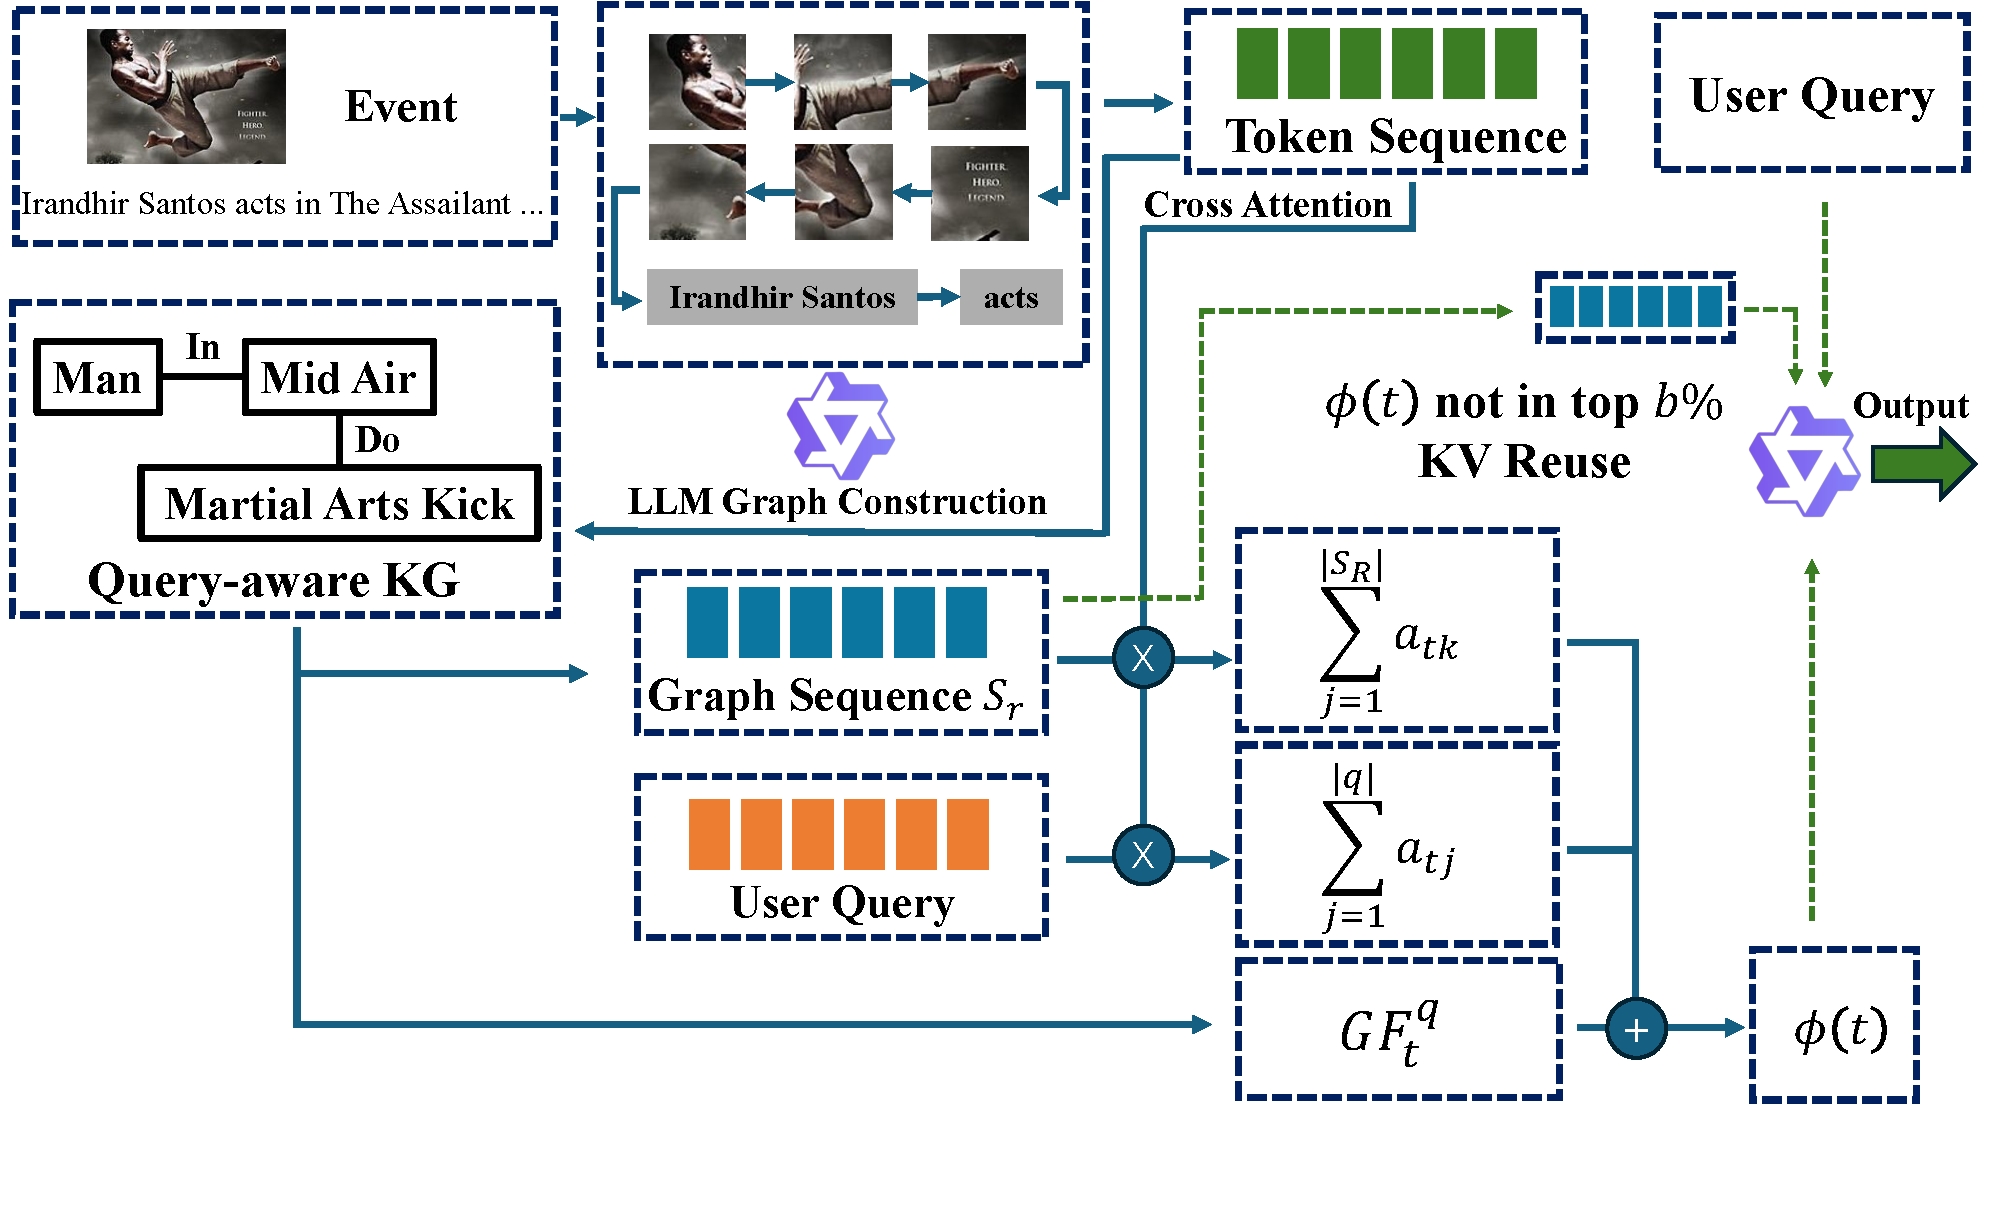
\includegraphics[width=0.95\textwidth]{figures/mgrag/graph_based_cache.pdf}
\caption{Graph features supplement attention in token recomputation scoring. The diagram retains the original graphical content. Original Figure 4, p.~2487~\cite{mgrag-paper}.}
\label{fig:mgrag:cache}
\end{figure}

\subsection{Topological features of facts}

MGRAG uses degree, betweenness, eigenvector, and closeness centrality to characterize a node. Degree centrality measures its normalized number of adjacent connections. Betweenness characterizes its participation in paths connecting other nodes. Eigenvector centrality weights connections by the centrality of their neighbors. Closeness uses distances to other graph nodes. The published method averages these four quantities,
\begin{equation}
 f(u)=\frac{dc(u)+bc(u)+ec(u)+cc(u)}{4}.
\label{eq:mgrag:node-feature}
\end{equation}
For a token associated with a triple $(u,r,v)$, its graph feature is the mean of the endpoint scores,
\begin{equation}
 GF_t^q=\frac{f(u)+f(v)}{2}.
\label{eq:mgrag:token-feature}
\end{equation}
The token-to-fact association follows the entity and relation token spans in the serialized representation. Tokens referring to the same fact therefore receive a shared structural component.

The graph feature concerns an entity's position in the query-specific graph. A node that connects several extracted facts can carry a different score from an isolated endpoint. Because extraction is query-dependent, the feature is calculated from a representation already selected for that query. Its meaning is relational importance within that graph, rather than a corpus-wide importance measure.

The published graphs are small, with fewer than twenty entities on average according to the report. Averaging four graph statistics provides a direct structural feature for these graphs. The recomputation score uses graph and attention information available during processing.

\subsection{Combined recomputation score}

Let $a_{tj}$ denote attention between token $t$ and token $j$, and let $|q|$ and $|S_r|$ denote the query and serialized-graph lengths. The score is
\begin{equation}
 \phi(t)=\sum_{j=1}^{|q|}a_{tj}
       +\sum_{k=1}^{|S_r|}a_{tk}+GF_t^q.
\label{eq:mgrag:cache-score}
\end{equation}
The first term expresses interaction with the current question. The second expresses interaction with the selected relational context. The third assigns the structural feature of the associated graph fact. The resulting sum determines which token states consume the recomputation budget.

The publication compares the policy with vLLM prefix caching~\cite{mgrag-kwon2023efficient} and CacheBlend~\cite{mgrag-yao2025cacheblend}. Their retrieval pipelines and cache variants are identified separately in the evaluation. The inverse ablations also evaluate graph-aware recomputation within an existing retrieval pipeline. These comparisons expose answer-quality and time changes under several compositions of retrieval and caching.

\section{Computational Cost}
\label{sec:mgrag:complexity}

The published offline encoding cost is $O(|\mathcal C|d_{\mathrm{emb}}l_c^2)$, with embedding dimension $d_{\mathrm{emb}}$. Using $k$ processed chunks, query-graph vertex and edge sets $\widehat{\mathcal V}$ and $\widehat{\mathcal E}$, evidence-graph sets $\mathcal V$ and $\mathcal E$, maximum path length $l_p$, and language-model hidden dimension $d_{\mathrm{LLM}}$, its reported online bound is
\begin{equation}
\begin{split}
 O\bigl(&d_{\mathrm{emb}}kl_c^2
 +l_p|\widehat{\mathcal E}|\,|\mathcal V|^{|\widehat{\mathcal V}|+1}
 +|\mathcal V||\mathcal E|\\
 &+d_{\mathrm{LLM}}(|S_r|^2+|q|^2)\bigr).
\end{split}
\label{eq:mgrag:complexity}
\end{equation}
The mapping-enumeration term is exponential in query-graph size. Query-specific construction and a bounded path length restrict the graphs processed in the evaluated setting. Actual module costs provide the complementary evidence about where runtime is spent. In particular, graph construction calls the language model repeatedly, whereas matching operates on the extracted graph. Section~\ref{sec:mgrag:cost-results} reports these costs individually.

\section{Experimental Protocol}
\label{sec:mgrag:protocol}

The evaluation uses MMQA~\cite{mgrag-talmor2021multimodalqa} and the Arxiv, Manual, Web, Wiki, Wit, and Recipe subsets of MRAMG-Bench~\cite{mgrag-yu2025mramg}. Table~\ref{tab:mgrag:datasets} preserves the published dataset statistics. MMQA includes textual and image queries. The six MRAMG subsets contain textual queries over multimodal corpora. Their query-hop ranges and corpus sizes differ, so results are reported by dataset.

\begin{table}[!htbp]
\centering
\small
\setlength{\tabcolsep}{3pt}
\caption{Evaluation datasets, reproduced from published Table 3, p.~2488~\cite{mgrag-paper}. T and I denote textual and image query modalities. The columns comprise MMQA and six MRAMG subsets.}\label{tab:mgrag:datasets}
\begin{tabular}{lccccccc}
\toprule
Statistic & MMQA & Wiki & Wit & Recipe & Arxiv & Manual & Web\\
\midrule
Query Modality     & T / I       & T             & T            & T               & T              & T               & T             \\
Queries            & 951           & 500           & 600          & 2,360            & 200            & 390             & 750           \\
Texts              & 218,285       & 538           & 639          & 1,528           & 101            & 40              & 1,500         \\
Images             & 57,058        & 538           & 639          & 8,569           & 337            & 2,607           & 1,500         \\
Corpus Size             & 22.5M        & 680k           & 478k          & 1.1M           & 136k            & 420k           & 215k         \\
Query Hops             & 1--2        & 2--5           & 2--4          & 1--6           & 3--4            & 2--6           & 2--3         \\
Avg Query Hops 	   & 1.5           & 3.0           & 2.8          & 3.3             & 3.1            & 3.7             & 2.4           \\
\bottomrule
\end{tabular}
\end{table}


The shared generation backbone is Qwen2.5-VL-7B-Instruct~\cite{mgrag-bai2025qwen2}. The experiments run on an Intel Xeon Gold 5220R CPU at 2.20 GHz and one NVIDIA A100-SXM4 GPU with 40 GB memory. The retrieval amount is set to five, text chunks use 256 tokens, and overlap is 32 tokens. HippoRAG2 uses Contriever for dense passage retrieval~\cite{mgrag-izacardunsupervised}; the other reported embedding configurations use bge-base-en-v1.5. Similarity-based retrieval represents images through their captions. These are the published controls for the comparisons in this chapter.

VanillaRAG is implemented with LangChain and FAISS~\cite{mgrag-douze2024faiss}. The GraphRAG implementation is nano-graphrag~\cite{mgrag-nanographrag}, and the remaining baseline systems use their released implementations. The protocol selects hybrid search for LightRAG and local search for GraphRAG. vLLM accelerates the tested baseline systems, while MGRAG uses its graph-aware cache procedure. Other baseline hyperparameters follow the implementations' defaults.

Four metrics characterize answers. Semantic similarity (SIM.) is the cosine similarity between bge-base-en-v1.5 representations of generated and reference answers. Accuracy (ACC.) is the reported proportion of correct answers. ROUGE-L (ROG.) evaluates longest-common-subsequence overlap~\cite{mgrag-lin2004rouge}, and BLEU-1 evaluates modified unigram precision~\cite{mgrag-papineni2002bleu}. The paper uses the RAGAS evaluation framework~\cite{mgrag-es2024ragas}. The tables preserve its metric names and precision, including the label BLEU used for BLEU-1.

The four answer metrics reflect different properties. Embedding similarity compares semantic proximity at the answer level. ROUGE-L and BLEU-1 retain sensitivity to the wording shared with the reference. Accuracy provides the task's correctness measurement. They are shown together because agreement in one measure does not imply identical behavior in the others. The publication reports point estimates for these experiments.

The complete-system baselines use different retrieval units. VanillaRAG returns dense-retrieved chunks, and R1-Searcher incorporates reinforcement learning into search and question answering. GraphRAG organizes its graph into communities and prepares summaries; LightRAG retrieves graph elements and neighborhoods through its selected search mode. HippoRAG2 adds passage nodes and uses Personalized PageRank for retrieval. In the published experiment, these systems are compared as implemented pipelines. Their results include their own indexing and evidence-selection choices, while the shared backbone and evaluation metrics provide the common answering conditions.

Component substitutions evaluate graph construction, semantic matching, and cache policy within MGRAG. Inverse ablations add matching and recomputation to other retrieval systems.

\section{Answer Quality and Structural Retrieval}
\label{sec:mgrag:results}

\subsection{Complete-system comparisons}

Table~\ref{tab:mgrag:main} reproduces the complete-system results. MGRAG has the highest reported value in each of the four metric rows for each dataset. On MMQA, its accuracy is 0.7442, compared with 0.7053 for VanillaRAG and 0.6335 for HippoRAG2. Its semantic similarity is 0.8533, ROUGE-L is 0.6763, and BLEU-1 is 0.7215. GraphRAG and LightRAG have missing MMQA entries because those experiments exceeded three days. The dash records the time limit and supplies no quality measurement for those systems.

{\small
\setlength{\tabcolsep}{3pt}
\begin{longtable}{llrrrrrr}
\caption{Answer quality with Qwen2.5-VL-7B-Instruct, reproduced from published Table 4, p.~2489~\cite{mgrag-paper}. Vanilla., R1., Graph., Light., and Hippo. denote VanillaRAG, R1-Searcher, GraphRAG, LightRAG, and HippoRAG2. A dash means that the experiment exceeded three days; it is not a zero score. Bold and underlining retain the publication's highlighting.}\label{tab:mgrag:main}\\
\toprule
Dataset & Metric & Vanilla. & R1. & Graph. & Light. & Hippo. & MGRAG\\
\midrule\endfirsthead
\multicolumn{8}{c}{\tablename\ \thetable\ (continued)}\\
\toprule
Dataset & Metric & Vanilla. & R1. & Graph. & Light. & Hippo. & MGRAG\\
\midrule\endhead
\bottomrule\endfoot
MMQA & SIM. & 0.8362 & 0.5478 & - & - & \underline{0.8381} & \textbf{0.8533} \\
MMQA & ACC. & \underline{0.7053} & 0.3567 & - & - & 0.6335 & \textbf{0.7442} \\
MMQA & ROG. & 0.5942 & 0.1041 & - & - & \underline{0.6659} & \textbf{0.6763} \\
MMQA & BLEU & \underline{0.6645} & 0.0817 & - & - & 0.5917 & \textbf{0.7215} \\
Arxiv & SIM. & \underline{0.8664} & 0.7051 & 0.7943 & 0.7404 & 0.8293 & \textbf{0.8760} \\
Arxiv & ACC. & \underline{0.6638} & 0.3775 & 0.2350 & 0.3813 & 0.4688 & \textbf{0.6800} \\
Arxiv & ROG. & \underline{0.2713} & 0.1189 & 0.1553 & 0.1580 & 0.2331 & \textbf{0.2726} \\
Arxiv & BLEU & \underline{0.2452} & 0.1092 & 0.1690 & 0.1370 & 0.1281 & \textbf{0.2498} \\
Manual & SIM. & \underline{0.8166} & 0.6046 & 0.5453 & 0.7255 & 0.6852 & \textbf{0.8221} \\
Manual & ACC. & \underline{0.5881} & 0.2071 & 0.1436 & 0.4096 & 0.2641 & \textbf{0.6173} \\
Manual & ROG. & \underline{0.3509} & 0.1078 & 0.0974 & 0.1595 & 0.2047 & \textbf{0.3839} \\
Manual & BLEU & \underline{0.2767} & 0.0740 & 0.0718 & 0.1385 & 0.1314 & \textbf{0.3093} \\
Web & SIM. & \underline{0.6937} & 0.6620 & 0.5470 & 0.5513 & 0.5642 & \textbf{0.7009} \\
Web & ACC. & \underline{0.4703} & 0.4200 & 0.1053 & 0.2000 & 0.3607 & \textbf{0.5123} \\
Web & ROG. & \underline{0.1508} & 0.1142 & 0.1133 & 0.0905 & 0.0616 & \textbf{0.1664} \\
Web & BLEU & 0.0326 & 0.0785 & \underline{0.1031} & 0.0206 & 0.0133 & \textbf{0.1456} \\
Wiki & SIM. & \underline{0.8824} & 0.5478 & 0.6966 & 0.7517 & 0.8204 & \textbf{0.8838} \\
Wiki & ACC. & \underline{0.7800} & 0.3567 & 0.2000 & 0.3660 & 0.6500 & \textbf{0.7845} \\
Wiki & ROG. & \underline{0.3559} & 0.1418 & 0.1361 & 0.2008 & 0.3042 & \textbf{0.3579} \\
Wiki & BLEU & \underline{0.3053} & 0.1146 & 0.1007 & 0.1863 & 0.1851 & \textbf{0.3174} \\
Wit & SIM. & \underline{0.7851} & 0.6110 & 0.6211 & 0.6973 & 0.7230 & \textbf{0.8033} \\
Wit & ACC. & \underline{0.6675} & 0.6017 & 0.1500 & 0.2483 & 0.5138 & \textbf{0.6967} \\
Wit & ROG. & \underline{0.3255} & 0.1307 & 0.1319 & 0.2416 & 0.2712 & \textbf{0.3589} \\
Wit & BLEU & \underline{0.2095} & 0.0934 & 0.1142 & 0.1928 & 0.1200 & \textbf{0.2382} \\
Recipe & SIM. & \underline{0.8599} & 0.6155 & 0.8166 & 0.8118 & 0.7792 & \textbf{0.8673} \\
Recipe & ACC. & \underline{0.6525} & 0.2180 & 0.2771 & 0.3334 & 0.4917 & \textbf{0.6814} \\
Recipe & ROG. & \underline{0.3714} & 0.1065 & 0.1745 & 0.2128 & 0.3303 & \textbf{0.4220} \\
Recipe & BLEU & \underline{0.2599} & 0.0773 & 0.1527 & 0.1648 & 0.1941 & \textbf{0.3102} \\
\end{longtable}
}


The advantage over the strongest baseline varies by dataset and metric. On Wiki, accuracy is 0.7845 for MGRAG and 0.7800 for VanillaRAG, while their semantic similarities are 0.8838 and 0.8824. On Web, the corresponding accuracies are 0.5123 and 0.4703. On Recipe, MGRAG reports ROUGE-L of 0.4220 compared with 0.3714 for VanillaRAG.

Several graph-based baselines score below VanillaRAG in this multimodal protocol. For example, on Manual, GraphRAG, LightRAG, and HippoRAG2 report accuracies of 0.1436, 0.4096, and 0.2641, compared with VanillaRAG's 0.5881. The presence of a graph by itself therefore does not predict the ranking in this table. MGRAG's results concern its specific construction, matching, and context-processing design. The substitutions below help identify which parts contribute under the same evaluation framework.

\subsection{Construction and matching substitutions}

Table~\ref{tab:mgrag:matching} reorganizes every value from the published graph-construction and matching comparison. Stanford OpenIE~\cite{mgrag-angeli2015leveraging} and the statistical extraction alternative STAT replace the construction mechanism. VF2 and ISMAGS~\cite{mgrag-cordella2004sub,mgrag-houbraken2014index} provide exact-matching alternatives. SM, VJ, RRWM, and IPFP represent approximate graph matching~\cite{mgrag-leordeanu2005spectral,mgrag-fankhauser2011speeding,mgrag-cho2010reweighted,mgrag-leordeanu2009integer}. BGE, SLOTAlign, and FGWAlign supply semantic alternatives~\cite{mgrag-bge_embedding,mgrag-tang2023robust,mgrag-tang2025fused}. The table preserves the publication's three-decimal precision for this experiment.

{\small
\setlength{\tabcolsep}{3pt}
\begin{longtable}{llrrrr}
\caption{Graph-construction and graph-matching substitutions, transposed from published Table 7, p.~2490~\cite{mgrag-paper}. All twelve method columns and all four metric values per dataset are retained. O.IE and STAT replace graph construction; the other alternatives replace matching. The shared backbone is Qwen2.5-VL-7B-Instruct. }\label{tab:mgrag:matching}\\
\toprule
Dataset & Method & SIM. & ACC. & ROG. & BLEU\\
\midrule\endfirsthead
\multicolumn{6}{c}{\tablename\ \thetable\ (continued)}\\
\toprule
Dataset & Method & SIM. & ACC. & ROG. & BLEU\\
\midrule\endhead
\bottomrule\endfoot
MMQA & O.IE & 0.642 & 0.571 & 0.510 & 0.483 \\
MMQA & STAT & 0.655 & 0.602 & 0.519 & 0.500 \\
MMQA & VF2 & 0.851 & 0.735 & 0.673 & 0.620 \\
MMQA & ISMAGS & 0.833 & 0.706 & 0.638 & 0.590 \\
MMQA & SM & 0.832 & 0.702 & 0.632 & 0.582 \\
MMQA & VJ & 0.812 & 0.715 & 0.646 & 0.606 \\
MMQA & RRWM & 0.838 & 0.698 & 0.647 & 0.599 \\
MMQA & IPFP & 0.773 & 0.633 & 0.601 & 0.585 \\
MMQA & BGE & 0.832 & 0.703 & 0.635 & 0.586 \\
MMQA & SLOT & 0.838 & 0.700 & 0.650 & 0.602 \\
MMQA & FGW & 0.837 & 0.697 & 0.647 & 0.598 \\
MMQA & MGRAG & 0.853 & 0.744 & 0.676 & 0.722 \\
\midrule
Arxiv & O.IE & 0.618 & 0.526 & 0.177 & 0.138 \\
Arxiv & STAT & 0.640 & 0.576 & 0.184 & 0.145 \\
Arxiv & VF2 & 0.871 & 0.650 & 0.270 & 0.239 \\
Arxiv & ISMAGS & 0.868 & 0.643 & 0.266 & 0.231 \\
Arxiv & SM & 0.866 & 0.670 & 0.263 & 0.244 \\
Arxiv & VJ & 0.872 & 0.667 & 0.269 & 0.245 \\
Arxiv & RRWM & 0.874 & 0.675 & 0.257 & 0.243 \\
Arxiv & IPFP & 0.814 & 0.581 & 0.212 & 0.203 \\
Arxiv & BGE & 0.874 & 0.668 & 0.270 & 0.244 \\
Arxiv & SLOT & 0.872 & 0.653 & 0.269 & 0.233 \\
Arxiv & FGW & 0.868 & 0.651 & 0.264 & 0.230 \\
Arxiv & MGRAG & 0.876 & 0.680 & 0.273 & 0.250 \\
\midrule
Manual & O.IE & 0.520 & 0.459 & 0.245 & 0.209 \\
Manual & STAT & 0.509 & 0.443 & 0.234 & 0.182 \\
Manual & VF2 & 0.817 & 0.612 & 0.377 & 0.306 \\
Manual & ISMAGS & 0.817 & 0.612 & 0.382 & 0.307 \\
Manual & SM & 0.813 & 0.614 & 0.378 & 0.303 \\
Manual & VJ & 0.808 & 0.608 & 0.372 & 0.298 \\
Manual & RRWM & 0.811 & 0.614 & 0.377 & 0.303 \\
Manual & IPFP & 0.800 & 0.594 & 0.369 & 0.289 \\
Manual & BGE & 0.815 & 0.615 & 0.375 & 0.303 \\
Manual & SLOT & 0.813 & 0.611 & 0.375 & 0.301 \\
Manual & FGW & 0.820 & 0.600 & 0.374 & 0.292 \\
Manual & MGRAG & 0.822 & 0.617 & 0.384 & 0.309 \\
\midrule
Web & O.IE & 0.466 & 0.290 & 0.052 & 0.020 \\
Web & STAT & 0.485 & 0.298 & 0.101 & 0.095 \\
Web & VF2 & 0.677 & 0.507 & 0.156 & 0.088 \\
Web & ISMAGS & 0.675 & 0.509 & 0.155 & 0.079 \\
Web & SM & 0.676 & 0.507 & 0.156 & 0.056 \\
Web & VJ & 0.679 & 0.508 & 0.160 & 0.056 \\
Web & RRWM & 0.675 & 0.503 & 0.157 & 0.066 \\
Web & IPFP & 0.666 & 0.493 & 0.149 & 0.055 \\
Web & BGE & 0.687 & 0.510 & 0.156 & 0.095 \\
Web & SLOT & 0.676 & 0.498 & 0.154 & 0.116 \\
Web & FGW & 0.676 & 0.480 & 0.147 & 0.096 \\
Web & MGRAG & 0.701 & 0.512 & 0.166 & 0.146 \\
\midrule
Wiki & O.IE & 0.504 & 0.498 & 0.230 & 0.200 \\
Wiki & STAT & 0.525 & 0.510 & 0.253 & 0.218 \\
Wiki & VF2 & 0.877 & 0.752 & 0.352 & 0.300 \\
Wiki & ISMAGS & 0.879 & 0.754 & 0.355 & 0.303 \\
Wiki & SM & 0.878 & 0.750 & 0.353 & 0.298 \\
Wiki & VJ & 0.873 & 0.751 & 0.349 & 0.297 \\
Wiki & RRWM & 0.878 & 0.743 & 0.355 & 0.301 \\
Wiki & IPFP & 0.869 & 0.735 & 0.348 & 0.296 \\
Wiki & BGE & 0.878 & 0.746 & 0.355 & 0.301 \\
Wiki & SLOT & 0.879 & 0.749 & 0.356 & 0.301 \\
Wiki & FGW & 0.878 & 0.747 & 0.352 & 0.300 \\
Wiki & MGRAG & 0.884 & 0.785 & 0.358 & 0.317 \\
\midrule
Wit & O.IE & 0.492 & 0.465 & 0.233 & 0.210 \\
Wit & STAT & 0.489 & 0.453 & 0.205 & 0.198 \\
Wit & VF2 & 0.799 & 0.693 & 0.354 & 0.234 \\
Wit & ISMAGS & 0.797 & 0.694 & 0.355 & 0.231 \\
Wit & SM & 0.784 & 0.686 & 0.353 & 0.229 \\
Wit & VJ & 0.786 & 0.691 & 0.356 & 0.227 \\
Wit & RRWM & 0.795 & 0.679 & 0.347 & 0.230 \\
Wit & IPFP & 0.792 & 0.678 & 0.346 & 0.231 \\
Wit & BGE & 0.789 & 0.689 & 0.356 & 0.230 \\
Wit & SLOT & 0.793 & 0.693 & 0.351 & 0.227 \\
Wit & FGW & 0.794 & 0.691 & 0.349 & 0.223 \\
Wit & MGRAG & 0.803 & 0.697 & 0.359 & 0.238 \\
\midrule
Recipe & O.IE & 0.551 & 0.425 & 0.211 & 0.202 \\
Recipe & STAT & 0.545 & 0.401 & 0.198 & 0.172 \\
Recipe & VF2 & 0.859 & 0.679 & 0.413 & 0.304 \\
Recipe & ISMAGS & 0.861 & 0.668 & 0.407 & 0.302 \\
Recipe & SM & 0.862 & 0.678 & 0.411 & 0.305 \\
Recipe & VJ & 0.857 & 0.672 & 0.413 & 0.295 \\
Recipe & RRWM & 0.852 & 0.670 & 0.406 & 0.298 \\
Recipe & IPFP & 0.847 & 0.661 & 0.395 & 0.221 \\
Recipe & BGE & 0.864 & 0.674 & 0.415 & 0.308 \\
Recipe & SLOT & 0.861 & 0.675 & 0.412 & 0.306 \\
Recipe & FGW & 0.860 & 0.677 & 0.409 & 0.305 \\
Recipe & MGRAG & 0.867 & 0.681 & 0.422 & 0.310 \\
\midrule
\end{longtable}
}


On MMQA, the full method reports accuracy 0.744, compared with 0.571 for OpenIE and 0.602 for STAT. These substitutions change the available extracted evidence. Their lower scores establish the importance of the evaluated construction choice for this setting. The evaluated extraction setting uses multimodal evidence and query-specific graphs.

Among MMQA matching alternatives, VF2 reaches accuracy 0.735, while MGRAG reaches 0.744. VF2 also has ROUGE-L of 0.673 compared with 0.676. On Web, BGE reaches accuracy 0.510 and MGRAG 0.512. On Wiki, ISMAGS reaches 0.754 and MGRAG 0.785. MGRAG leads the displayed metric rows, with smaller MMQA and Web accuracy margins than the Wiki accuracy margin.

\subsection{Queries requiring multiple hops}

Table~\ref{tab:mgrag:hops} reports results grouped by MRAMG query-hop count. For one-hop questions, VanillaRAG reports accuracy 0.613 and MGRAG 0.624. For six-hop questions, the reported values are 0.661 and 0.738. MGRAG also reports higher ROUGE-L and BLEU-1 for each hop group. The table's time entries favor VanillaRAG throughout: the one-hop values are 0.13 and 0.35 minutes, and the six-hop values are 0.18 and 0.43 minutes.

{\small
\setlength{\tabcolsep}{3pt}
\begin{longtable}{lrlrrrr}
\caption{Results by query hop count, reorganized from published Table 8, p.~2490~\cite{mgrag-paper}. Time is in minutes, as reported. Each original row is shown as two method rows, with the query count repeated.}\label{tab:mgrag:hops}\\
\toprule
Hops & Queries & Method & Time & ACC. & ROG. & BLEU\\
\midrule\endfirsthead
\multicolumn{7}{c}{\tablename\ \thetable\ (continued)}\\
\toprule
Hops & Queries & Method & Time & ACC. & ROG. & BLEU\\
\midrule\endhead
\bottomrule\endfoot
1-hop & 201 & VanillaRAG & \textbf{0.13} & 0.613 & 0.379 & 0.240 \\
1-hop & 201 & MGRAG & 0.35 & \textbf{0.624} & \textbf{0.425} & \textbf{0.286} \\
2-hop & 1,237 & VanillaRAG & \textbf{0.10} & 0.588 & 0.304 & 0.193 \\
2-hop & 1,237 & MGRAG & 0.37 & \textbf{0.601} & \textbf{0.335} & \textbf{0.230} \\
3-hop & 2,357 & VanillaRAG & \textbf{0.16} & 0.633 & 0.329 & 0.238 \\
3-hop & 2,357 & MGRAG & 0.41 & \textbf{0.659} & \textbf{0.355} & \textbf{0.260} \\
4-hop & 499 & VanillaRAG & \textbf{0.19} & 0.697 & 0.338 & 0.259 \\
4-hop & 499 & MGRAG & 0.44 & \textbf{0.712} & \textbf{0.373} & \textbf{0.293} \\
5-hop & 286 & VanillaRAG & \textbf{0.18} & 0.678 & 0.319 & 0.205 \\
5-hop & 286 & MGRAG & 0.45 & \textbf{0.733} & \textbf{0.392} & \textbf{0.282} \\
6-hop & 220 & VanillaRAG & \textbf{0.18} & 0.661 & 0.305 & 0.176 \\
6-hop & 220 & MGRAG & 0.43 & \textbf{0.738} & \textbf{0.377} & \textbf{0.249} \\
\end{longtable}
}


The six-hop group contains 220 queries, whereas the three-hop group contains 2,357. These group sizes matter when interpreting the distribution of the evidence. The comparison shows a larger accuracy gap on the longest-hop group than on the shortest-hop group, alongside additional processing time. It supplies a direct account of the quality-cost trade-off for questions with different relational demands.

\section{Cache Quality and End-to-end Costs}
\label{sec:mgrag:cost-results}

Table~\ref{tab:mgrag:cache} preserves the MMQA cache-system comparison. MGRAG reports accuracy 0.7442 and total time 4.3 hours. The vLLM and CacheBlend variants paired with VanillaRAG report accuracies 0.6593 and 0.6601, with total time 4.5 hours for both. Paired with HippoRAG2, they report accuracies 0.6335 and 0.6267, with total times of 8.8 and 8.3 hours. These are distinct retrieval-and-cache compositions, each identified in the table.

{\small
\setlength{\tabcolsep}{3pt}
\begin{longtable}{lrrrrrr}
\caption{Cache-system comparison on MMQA, reproduced from published Table 6, p.~2489~\cite{mgrag-paper}. V. and H. identify VanillaRAG and HippoRAG2 retrieval pipelines. TTFT is in seconds and total time is in hours.}\label{tab:mgrag:cache}\\
\toprule
System & SIM. & ACC. & ROG. & BLEU & TTFT & Time\\
\midrule\endfirsthead
\multicolumn{7}{c}{\tablename\ \thetable\ (continued)}\\
\toprule
System & SIM. & ACC. & ROG. & BLEU & TTFT & Time\\
\midrule\endhead
\bottomrule\endfoot
vLLM (V.) &          0.8315 & 0.6593 & 0.6277 & {0.5867}
&      \underline{3.2 s}         &     \underline{4.5 h}                \\
CacheBlend (V.)     &        0.8315       &      \underline{0.6601}         &       0.6417        &         \underline{0.5964}     &       \textbf{3.1 s}        &     \underline{4.5 h}                \\
vLLM (H.) &     0.8381     & 0.6335 & \underline{0.6659} & 0.5917
&          4.6 s    &         8.8 h            \\
CacheBlend (H.)     &      \underline{0.8415}     &     0.6267       &        0.6636       &      0.5917    &     4.4 s  &      8.3 h   \\
\textbf{MGRAG}           & \textbf{0.8533}        &\textbf{0.7442}        & \textbf{0.6763}        & \textbf{0.7215}        &        \underline{3.2 s}       & \textbf{4.3 h}                \\
\end{longtable}
}


Time to first token (TTFT) gives a different view from total time. CacheBlend with VanillaRAG reports 3.1 seconds, while MGRAG and vLLM with VanillaRAG report 3.2 seconds. MGRAG combines the highest answer-quality values with a total time of 4.3 hours; CacheBlend with VanillaRAG has the shortest TTFT. The two latency measures should be read alongside their quality measurements, because a system can change one without changing the other in the same direction.

The inverse-ablation table also measures quality when graph-aware recomputation is added after path matching. Within the HippoRAG2 composition, accuracy changes from 0.7372 with path matching to 0.7442 with both components, while the total time changes from 4.1 to 4.3 hours. The additional computation is accompanied by changes in answer quality. Its purpose is to allocate repeated computation to token states selected by the combined score.

Section~\ref{sec:mgrag:ablations} compares these component additions within the HippoRAG2 and VanillaRAG pipelines.

Table~\ref{tab:mgrag:breakdown} reports time and token costs by module. On MMQA, graph construction accounts for 193.0 minutes, matching for 0.14 minutes, and answer generation for 8.9 minutes; the reported end-to-end time is 248.1 minutes. The construction and generation token entries are 3,085 and 1,431, with end-to-end token entry 4,516. The listed module times do not sum to the reported end-to-end total; the publication does not reconcile the difference in this breakdown.

{\small
\setlength{\tabcolsep}{3pt}
\begin{longtable}{lrrrrr}
\caption{Module costs reproduced from published Table 5, p.~2489~\cite{mgrag-paper}. Time is in minutes. KGC, QA, and E2E cells retain the published time/token pairs for graph construction, answering, and end-to-end processing. Match denotes matching time. Token counts and E2E totals are preserved as reported.}\label{tab:mgrag:breakdown}\\
\toprule
Dataset & Queries & KGC & Match & QA & E2E\\
\midrule\endfirsthead
\multicolumn{6}{c}{\tablename\ \thetable\ (continued)}\\
\toprule
Dataset & Queries & KGC & Match & QA & E2E\\
\midrule\endhead
\bottomrule\endfoot
MMQA             & 951               & 193.0 / 3,085 & 0.14           & 8.9 / 1,431  & 248.1 / 4,516   \\
Arxiv            & 200               & 61.9 / 3,946  & 0.23           & 16.2 / 2,944  & 83.9 / 6,890    \\
Manual           & 390               & 76.1 / 4,285  & 0.04           & 23.9 / 2,556 & 109.7 / 6,841    \\
Web              & 750               & 143.8 / 4,623  & 0.27           & 42.9 / 3,101 & 196.5 / 7,723   \\
Wiki             & 500               & 164.2 / 6,629  & 0.30           & 52.1 / 6,267 & 241.5 / 12,896  \\
Wit              & 600               & 140.6 / 7,660  & 0.21           & 42.6 / 6,539 & 196.5 / 14,199  \\
Recipe           & 2,360             & 525.7 / 4,351 & 1.74           & 191.3 / 3,173 & 808.7 / 7,525   \\
\end{longtable}
}


Graph construction is the largest listed time component on all seven datasets. Recipe reports 525.7 minutes for construction, 1.74 for matching, and 191.3 for answering, with end-to-end time 808.7 minutes. On the smaller Arxiv query set, the corresponding values are 61.9, 0.23, and 16.2 minutes, with end-to-end time 83.9. These measurements locate repeated extraction calls as a substantial cost within the evaluated pipeline, even though graph matching has an exponential worst-case bound.

The distinction between computational bounds and measured module costs is useful here. The graphs are built from query-selected evidence, so the matcher processes small instances in these experiments. Construction invokes the multimodal model on the selected chunks. Reducing the number of extracted chunks or the cost of each extraction could therefore affect the observed runtime substantially. Such changes are prospective design directions; the table records the published pipeline's cost.

\section{Ablations and Parameter Sensitivity}
\label{sec:mgrag:ablations}

\subsection{Component ablations}

The MMQA ablations in Table~\ref{tab:mgrag:ablation} change matching, coarse encoding, and pipeline composition. Removing graph matching constructs the query-specific graph from a fixed number of chunks and reports accuracy 0.7260, compared with 0.7442 for MGRAG. Replacing caption-based coarse ranking with direct CLIP encoding~\cite{mgrag-radford2021learning} reports accuracy 0.7376. The Vanilla MGRAG variant applies path matching and graph-aware caching within the VanillaRAG pipeline with $k=5$; it reports accuracy 0.6887.

{\small
\setlength{\tabcolsep}{3pt}
\begin{longtable}{lrrrrr}
\caption{MMQA component ablations, reproduced from published Table 9, p.~2490~\cite{mgrag-paper}. For Vanilla MGRAG, $k$ is the retrieval amount. Time is in hours.}\label{tab:mgrag:ablation}\\
\toprule
Model & SIM. & ACC. & ROG. & BLEU & Time\\
\midrule\endfirsthead
\multicolumn{6}{c}{\tablename\ \thetable\ (continued)}\\
\toprule
Model & SIM. & ACC. & ROG. & BLEU & Time\\
\midrule\endhead
\bottomrule\endfoot
Without graph matching        & 0.8362          & 0.7260          & 0.6657          & 0.5774          & \underline{4.4 h}       \\
With CLIP encoder  & \underline{0.8513}  & \underline{0.7376}  & \underline{0.6744}  & \underline{0.7008}  & 4.5 h               \\
Vanilla MGRAG, $k=5$         &           0.8260      &    0.6887             &         0.6266        &            0.5773     &       4.7 h              \\
\textbf{MGRAG} & \textbf{0.8533} & \textbf{0.7442} & \textbf{0.6763} & \textbf{0.7215} & \textbf{4.3 h}      \\
\end{longtable}
}


The full system also has the largest SIM., ROUGE-L, and BLEU-1 entries in this table. Its reported time is 4.3 hours, compared with 4.4 hours without graph matching, 4.5 hours with CLIP, and 4.7 hours for Vanilla MGRAG. The comparison supports the particular coarse-to-fine composition used in the published system. It also identifies the scope of the encoder observation: caption-based ranking performs better than the tested CLIP substitution on MMQA with this pipeline and backbone.

\subsection{Adding components to other pipelines}

Table~\ref{tab:mgrag:inverse} retains the inverse ablations. Adding graph-aware KV recomputation to HippoRAG2 changes accuracy from 0.6335 to 0.6855 and time from 7.5 to 7.6 hours. Adding path-based semantic matching gives accuracy 0.7372 and time 4.1 hours. Combining both gives accuracy 0.7442 and time 4.3 hours. The latter configuration shares MGRAG's reported values because the publication identifies its retrieval and generation setting with the full method once both components are incorporated.

\begin{table}[!htbp]
\centering
\small
\setlength{\tabcolsep}{3pt}
\caption{MMQA inverse ablations, reproduced from published Table 10, p.~2491~\cite{mgrag-paper}. PSGM and GKV denote path-based semantic graph matching and graph-aware KV recomputation. Time is in hours.}\label{tab:mgrag:inverse}
\begin{tabular}{lrrrrr}
\toprule
Model & SIM. & ACC. & ROG. & BLEU & Time\\
\midrule
Hippo.            & 0.8381          & 0.6335          & 0.6659          & 0.5917          & 7.5 h           \\
Hippo.+GKV        & 0.8392          & 0.6855          & 0.6651          & 0.7013          & 7.6 h           \\
Hippo.+PSGM       & 0.8416          & \underline{0.7372}  & \underline{0.6720}  & \underline{0.7128}  & \underline{4.1 h}   \\
Hippo.+PSGM+GKV   & \textbf{0.8533} & \textbf{0.7442} & \textbf{0.6763} & \textbf{0.7215} & 4.3 h           \\
\midrule
Vanilla.          & 0.8362          & 0.7053          & 0.5942          & 0.6645          & \textbf{2.6 h}  \\
Vanilla.+PSGM     & 0.8460          & 0.7175          & 0.6466          & 0.6973          & 4.7 h           \\
Vanilla.+PSGM+GKV & \underline{0.8485}  & 0.7232          & 0.6563          & 0.7001          & 4.8 h           \\
\midrule
\textbf{MGRAG}    & \textbf{0.8533} & \textbf{0.7442} & \textbf{0.6763} & \textbf{0.7215} & 4.3 h           \\
\bottomrule
\end{tabular}
\end{table}


For VanillaRAG, the base accuracy is 0.7053 at 2.6 hours. Adding path matching gives 0.7175 at 4.7 hours, and adding graph-aware recomputation as well gives 0.7232 at 4.8 hours. Thus, the component additions increase quality in these measured compositions, while their time changes depend on the host pipeline. The HippoRAG2 and VanillaRAG results make that dependence visible. They also distinguish the value of a component from the full system's overall comparison.

\subsection{Matching threshold and path length}

Figure~\ref{fig:mgrag:sensitivity} reproduces the published parameter curves. The experiments vary the semantic threshold $\theta$ and maximum path length $l_p$, including lengths $1,2,3$, and unrestricted length. The reported discussion identifies $\theta=0.6$ and $l_p=3$ as effective choices in these tests. 

\begin{figure}[tbp]
\centering
\begin{subfigure}{0.48\textwidth}
\centering
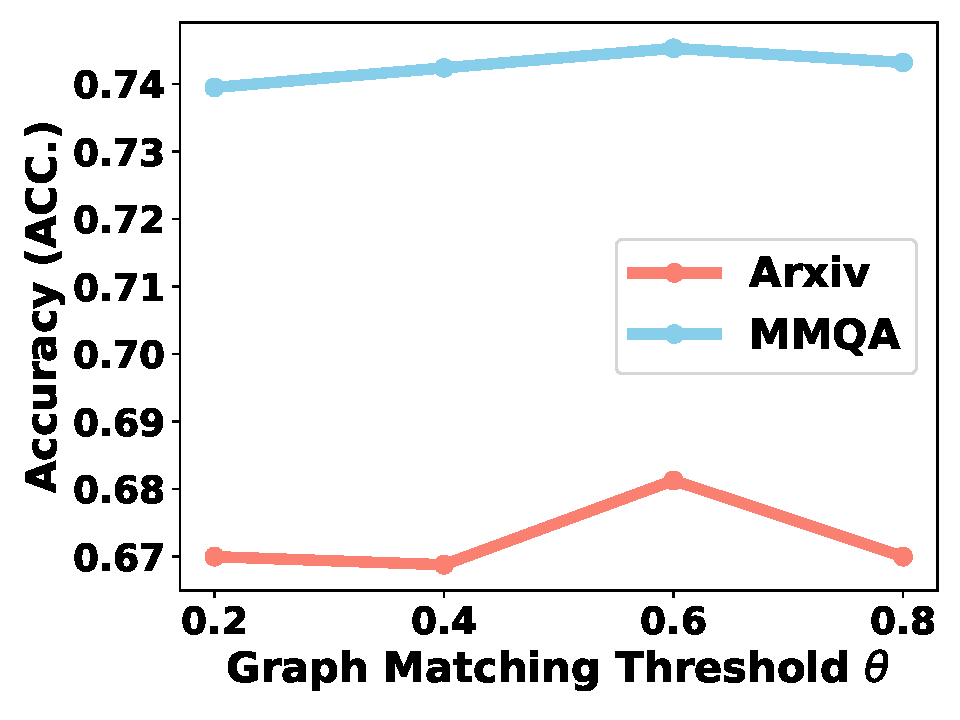
\includegraphics[width=\linewidth]{figures/mgrag/acc_vs_theta_fixed_lp.pdf}
\caption{Similarity threshold $\theta$.}
\end{subfigure}\hfill
\begin{subfigure}{0.48\textwidth}
\centering
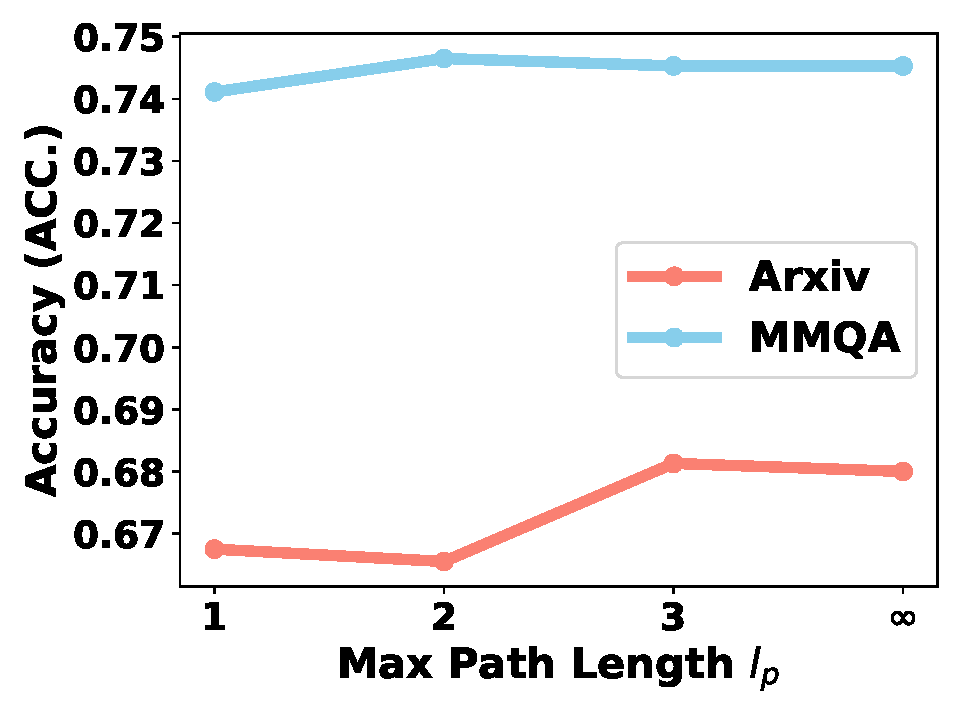
\includegraphics[width=\linewidth]{figures/mgrag/acc_vs_lp_fixed_theta.pdf}
\caption{Maximum path length $l_p$.}
\end{subfigure}
\caption{MGRAG matching-parameter sensitivity. Original subfigures of Figure 5, p.~2491~\cite{mgrag-paper}.}
\label{fig:mgrag:sensitivity}
\end{figure}

The threshold changes which entity correspondences and path extensions can pass validation. A higher value demands closer embedding agreement, while a lower value permits more candidates. The path-length cap determines how many relations may be used to express a query relation. Its effect therefore concerns both representational flexibility and search. These roles explain why the two parameters belong to the matching mechanism, while their empirical choice remains tied to the reported evaluation.

\section{Discussion and Chapter Summary}
\label{sec:mgrag:discussion}

MGRAG gives structure three connected responsibilities. Query-aware extraction determines which facts enter the graph. Path-based matching determines whether those facts express the relational requirements of the query. Graph features then influence the selection of token states for recomputation. The graph is consequently involved in constructing, selecting, and processing evidence, rather than serving only as a store from which a fixed number of items is retrieved.

The experiments support this design at several levels. Complete-system results report the highest values across the seven datasets' four answer metrics. Construction and matching substitutions evaluate the evidence representation and correspondence choices. The hop-group comparison shows additional quality gains for questions requiring more relational steps, together with added time. Cache comparisons and inverse ablations retain the context-serving contribution and expose its dependence on the surrounding retrieval pipeline.

Several conditions delimit the interpretation. Captions influence the coarse order of image evidence, and model-generated extraction determines which facts are available for matching. A valid semantic match is assessed against the extracted query graph and an embedding threshold; answer correctness is evaluated downstream. The maximum construction and path budgets restrict the search. The published runtime measurements use one hardware and model configuration, and the tables do not provide the fixed numerical recomputation budget needed to attribute a cost to a particular $b$ value. These conditions identify the representation and computation choices on which the reported results depend.

For the thesis's central question, the chapter establishes a concrete extension from connected textual evidence to query-dependent multimodal evidence. Semantic paths allow relations to be represented at different granularities across the query and evidence graphs. Selective KV recomputation shows a further use of the retrieved structure in context processing. The following discussion compares these roles with the representations and retrieval objects studied in KGLink, GORAG, and AGRAG, using their respective tasks and published evidence.
